\section{Taxonomic corrections}
Across the different sources, similar species could appear under different binomial names. This was a problem when matching datasets by species. Moreover, it is possible that within a source, a given species was appearing under two or more different, synonymic names. As such, taxonomic synonymy created duplicated rows for the same species, overall falsely increasing the total number of species and potentially inflating the number of missing trait values. Taxonomic synonymy was hence a major issue. Due to the large number of species across datasets, extensive manual checks could not be applied. The presence of typos in species names had the same effect as synonymy, erroneously duplicating species. We attempted to correct for taxonomy first by correcting for typos, and second by identifying species which were entered under non-accepted names and replacing these with the accepted name. To this end, we developed an automated procedure, complemented with a few manual entries where errors were opportunistically spotted. Such errors in taxonomy were notably spotted when attempting to retrieve trait data for subsets of species, for analyses unrelated to the work conducted here. Taxonomic synonymy was as such checked manually for 91 species (56 birds, 7 mammals and 28 reptiles); in that case, information was extracted from other diverse sources (such as the Reptile Database (\url{http://www.reptile-database.org/}); Avibase (\url{https://avibase.bsc-eoc.org/avibase.jsp?lang=EN\&pg=home}); AmphibiaWeb (\url{https://amphibiaweb.org/}); and additional manual checks using the IUCN Red List for mammals). A column in the Synonym dataset mentions where manual checks were applied (in which case the Synonym dataset was manually corrected). 


\subsection*{Automated procedure and outputs.}
\paragraph{Extracting names from the IUCN Red List and the Integrated Taxonomic Information System (ITIS).}
The objectives of the automated procedure were to (1) extract species synonymic binomial names from the IUCN Red List or from ITIS (using the rredlist \citep{rredlist} and taxize \citep{Chamberlain2013} R packages); and (2) identify the status of each name (accepted or not accepted). We started by generating a list of all names featuring in any of the sources. These `original' names were corrected for typos (using gnr$\textunderscore$resolve function, taxize package). Then, the IUCN Red List was queried and any listed synonyms were stored, as well as the status of each synonym (accepted or not accepted). When species were not found in the IUCN Red List, synonyms were extracted from ITIS. When species were not found in ITIS either, corrected names (original names corrected for typos) were used. Family and order designations were extracted using the same procedure and some entries were retrieved from the Global Biodiversity Information Facility taxonomic backbone when not available in the Red List or in the ITIS (GBIF, \url{https://www.gbif.org/tools/species-lookup}).\\
\textbf{NB:} for species entered with the forms \textit{Genus cf.}, \textit{Genus aff.} or \textit{Genus spp.}, the accepted binomial name was left empty.

\paragraph{Output.} We generated a `Synonym' dataset containing records of all names (for 14124, 8743, 6090, and 11678 binomial names for birds, amphibians, mammals and reptiles respectively), their status and their potential synonyms.

\paragraph{Harmonising taxonomy in trait datasets.}
Taxonomy across datasets was finally homogenised by replacing synonyms with a uniquely identified accepted name. As a consequence, the total number of identified unique species decreased (Figure \ref{SI2_taxcor} A). The species presenting the highest number of synonyms was the East African mole rat (\textit{Tachyoryctes splendens}), for which we found 12 synonymic names (Figure \ref{taxcor} B).

% figure: distribution of names and differences in species number
\vspace{0.5cm}
\begin{figure}[h!]
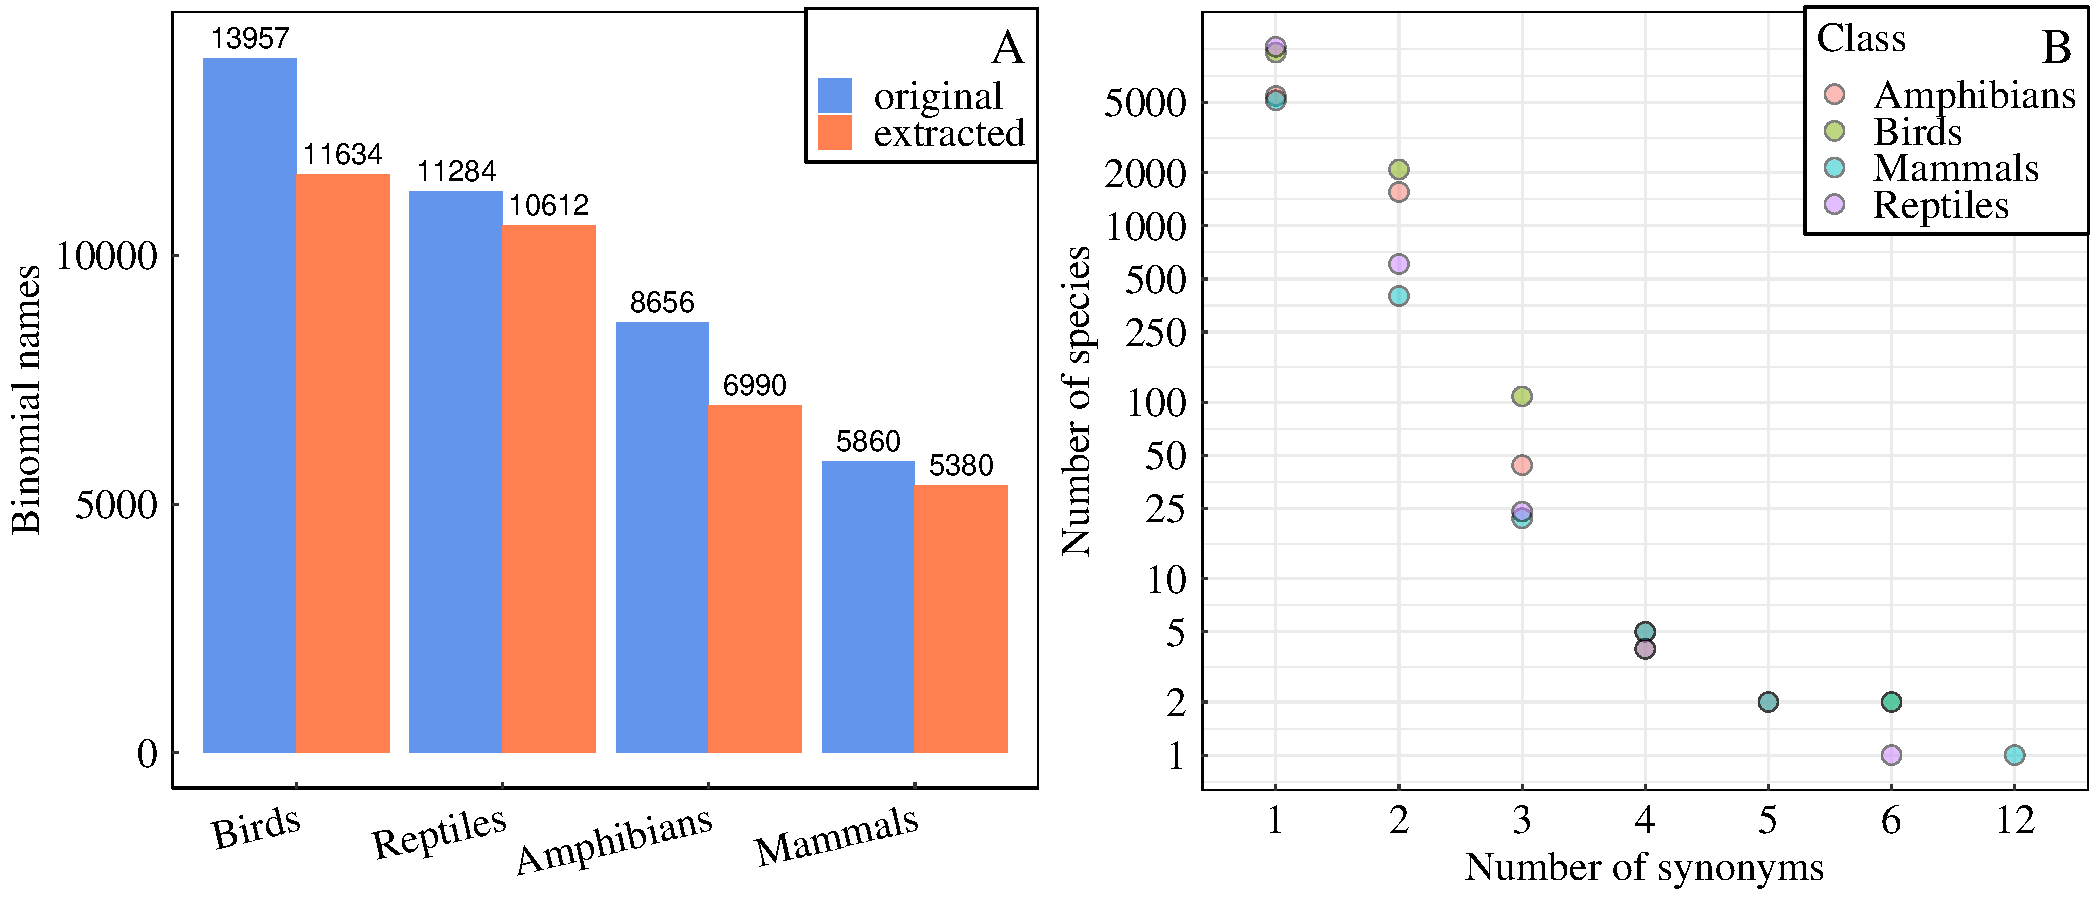
\includegraphics[scale=0.45]{Supporting/Chapter2/Figures/tax_corrections}
\caption[Difference in species number before and after taxonomic correction (A) and distribution of number of synonyms across datasets (B)]{\textbf{Difference in species number before and after taxonomic correction (A) and distribution of number of synonyms across datasets (B).} \textbf{(A)} shows the number of species (binomial names) extracted from all sources (blue bars), and the number of uniquely identified accepted names (in red). Replacing non-accepted synonyms by one identified accepted name reduced the number of species in all classes, with the largest reduction for birds. \textbf{(B)} shows the distribution of the number of synonymic names. In all four classes, more than 5,000 species were known under one name only. Nevertheless, a large number of species had two identified synonyms (range: 400 species for mammals - 2086 for birds). The most potentially replicated species was the East African mole rat \textit{Tachyoryctes splendens}, for which 12 synonyms were identified.}
\label{SI2_taxcor}
\end{figure}

%Decrease by 2,323 unique binomial names for birds. The diminution was of 632 unique identified species for reptiles, of 1,666 for amphibians and of 488 for mammals.

The automated procedure was not perfect, and taxonomic errors are likely to have persisted in the trait datasets. The Red List and the ITIS were not comprehensive taxonomic sources, and for clades with high degrees of synonymy in names, such as reptiles or amphibians, neither the Red List or the ITIS contained enough information.Taxonomy may be further improved by using class-specific sources in an automated procedure. 

\clearpage

\section{Additional information for trait compilation}

\begin{comment}
\subsection{Data sources for the `Senior' dataset}

\cite{Anderson1999} \\
\cite{Ao2003} \\
\cite{Arroyo2008} \\
\cite{Bain2004}\\
\cite{Barrio-Amoros2012}\\
\cite{Bennett1999} \\
\cite{Bernarde2009} \\
\cite{Blomquist2009} \\
\cite{Brasileiro2005} \\
\cite{Campbell1998} \\
\cite{Caramaschi1997} \\
\cite{DaSilva2009}\\ 
\cite{DeAlmeidaPrado2000} \\
\cite{DeAlmeidaPrado2003} \\
\cite{DeCarvalho2010} \\
\cite{Fouquet2007} \\
\cite{Goldberg2008} \\
\cite{Gonzalez2008} \\
\cite{Guayasamin2006} \\
\cite{Hertz2012}\\
\cite{Heyer1994} \\
\cite{Heyer1996} \\
\cite{Heyer2002} \\
\cite{Ibanez2012}\\
\cite{Jared2011} \\
\cite{Jungfer2002} \\
\cite{Kan2010} \\
\cite{Lance1993} \\
\cite{Lynch1989} \\
\cite{Matson1990} \\
\cite{McCranie1993} \\
\cite{Ningombam2007} \\
\cite{Ohler2011} \\
\cite{PombalJr.2011} \\
\cite{Savage2002} \\
\cite{Shahriza2010} \\
\cite{Shepard2005}\\
\cite{Simoes2010} \\
\cite{Stuart2006} \\
\cite{Su2005} \\
\cite{Sunyer2009} \\
\cite{Wollenberg2006} \\
\cite{Zimmermann1983} \\
\cite{Zug1979}\\
http://amphibia.my/\\
http://amphibiaweb.org/

\end{comment}


\subsection*{Correlations among closely related traits}

% Amphibians: body mass VS body length and Maturity VS longevity
\begin{figure}[h!]
\centering
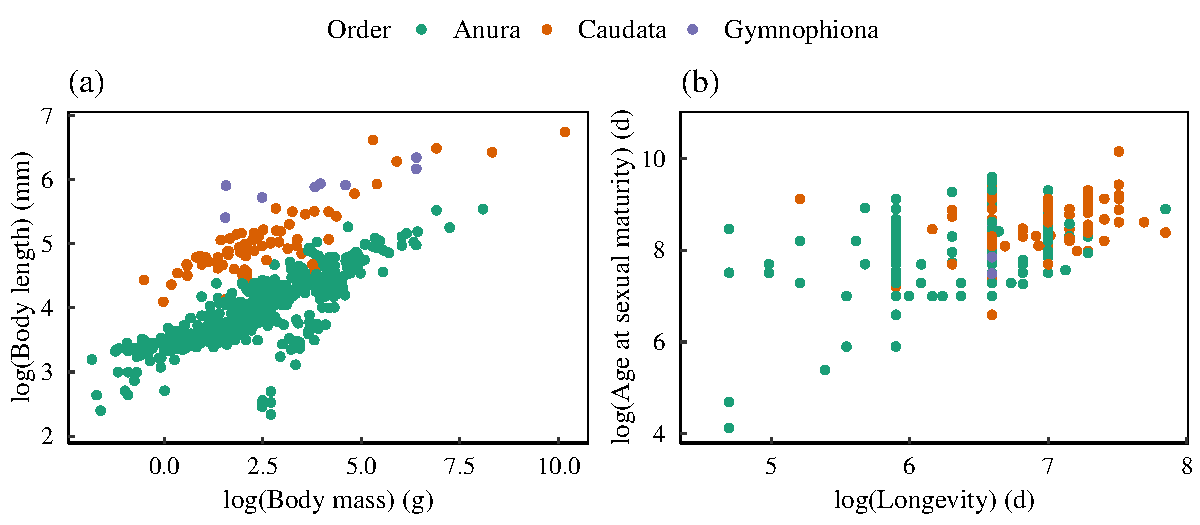
\includegraphics[scale=0.85]{Supporting/Chapter2/Figures/Correlations/MatLong_BMBL_amphibians}
\caption[(a) Body mass versus body length and (b) Longevity versus age at sexual maturity in amphibians.]{\textbf{(a) Body mass versus body length and (b) Longevity versus age at sexual maturity in amphibians.} The Pearson's correlation coefficient was 0.71 in (a) and 0.55 in (b) (order was not included in these coefficients).} 
\label{}
\end{figure}

% Birds: Longevity VS Generation length
\begin{figure}[h!]
\centering
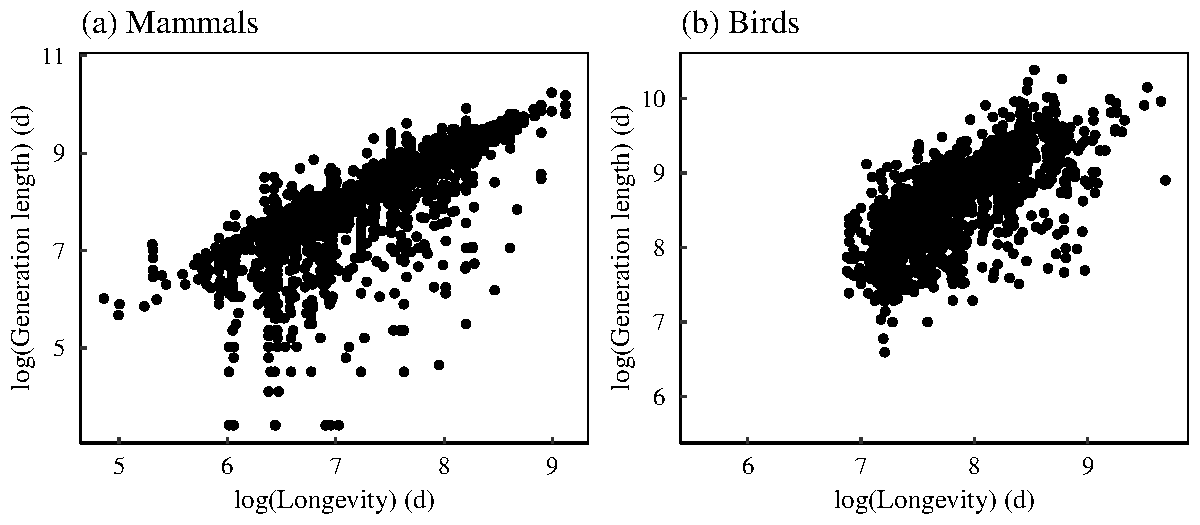
\includegraphics[scale=0.85]{Supporting/Chapter2/Figures/Correlations/GL_Longe_birds_mammals}
\caption[Generation length versus longevity data in birds.]{\textbf{Generation length versus longevity data in mammals and birds.} The Pearson's correlation coefficient was 0.74 in (a) and 0.70 in (b).} 
\label{}
\end{figure}

\pagebreak

\begin{comment}
\subsection{Habitat affinities and use of artificial habitats}

\paragraph{Habitat breadth.}
The IUCN Red List habitat data records habitat types in which species are found to occur. Habitats are classified into 96 categories, which we pooled into 13 broader habitat variables: 
Forest, Savanna, Grassland, Shrubland, Wetland, Rocky areas, Caves and subterranean, Desert, Marine, Marine intertidal or coastal/supratidal, Artificial, Introduced vegetation and Other/Unknown (level two of the IUCN Habitat Classification Scheme). Species habitat preferences were described using these variables as binary (taking 1 if a species was known to occur in the habitat and 0 otherwise). Habitat breadth was then calculated as the number of habitats recorded to be used by a species. Information regarding habitat suitability and habitat importance is also available in the IUCN Red List habitat data, so it is possible to use a weighted sum to calculate habitat breadth. Weights can be assigned to account for the suitability and importance of each habitat.
%Suitability was classified in three categories in the IUCN Red List: `suitable', `marginal' or  `unknown'. Suitable habitats were recorded to be either of major importance, not of major importance or of unknown importance. We used the weights provided in Table \ref{weights} to produce weighted sums of the number of habitats used by each species. Note that the weighting system used in this work does not impact coverage or completeness (as the amount of information across species remains similar regardless of the weights). Moreover, habitat breadth was not highly sensitive to the choice of weights (see Figure.)

% table of weigths used for habitat breadth calculations
\begin{table}[h!]
\renewcommand{\baselinestretch}{1}
\renewcommand{\arraystretch}{1.5}
\begin{center}\fontsize{9}{11}\selectfont
\caption[Weights used in the calculation of habitat breadth]{\textbf{Weights used in the calculation of habitat breadth.} Habitat breadth was calculated as the weighted sum of the number of habitats used by a species. Weights were assigned to each habitat given its importance and its suitability.} 
\label{weights}
\begin{tabular}{|l|c|c|c|}
\hline
\multicolumn{1}{|c|}{\multirow{2}{*}{\textbf{Suitability}}} & \multicolumn{3}{c|}{\textbf{Major importance}} \\ \cline{2-4} 
\multicolumn{1}{|c|}{}                             & \textbf{Yes}       & \textbf{No}        & \textbf{Unknown}       \\ \hline
\textbf{Suitable}                                           & 1         & 0.5       & 1             \\ \hline
\textbf{Marginal}                                           & NA       & 0.3       & 0.3           \\ \hline
\textbf{Unknown}                                            & NA         & 0.3       & 1             \\ \hline
\end{tabular}
\end{center}
\end{table}

\end{comment}

\clearpage

\section{Cutting distribution maps by altitudinal limits}

\begin{figure}[h!]
\centering
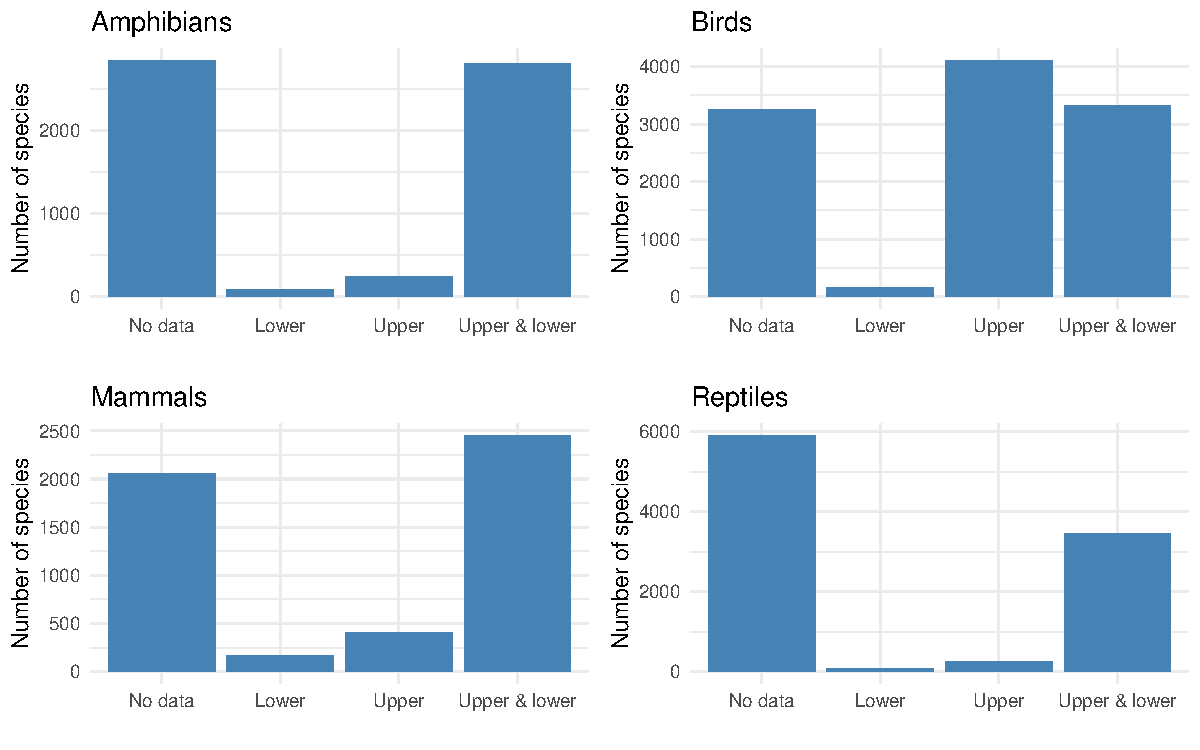
\includegraphics[scale=0.7]{Supporting/Chapter2/Figures/Rangesizes/Elevation_data_amount}
\caption[]{\textbf{Availability of altitudinal limits across species.} Upper and lower altitudinal limits were extracted from the IUCN Red List.}
\label{}
\end{figure}

\begin{figure}[h!]
\centering
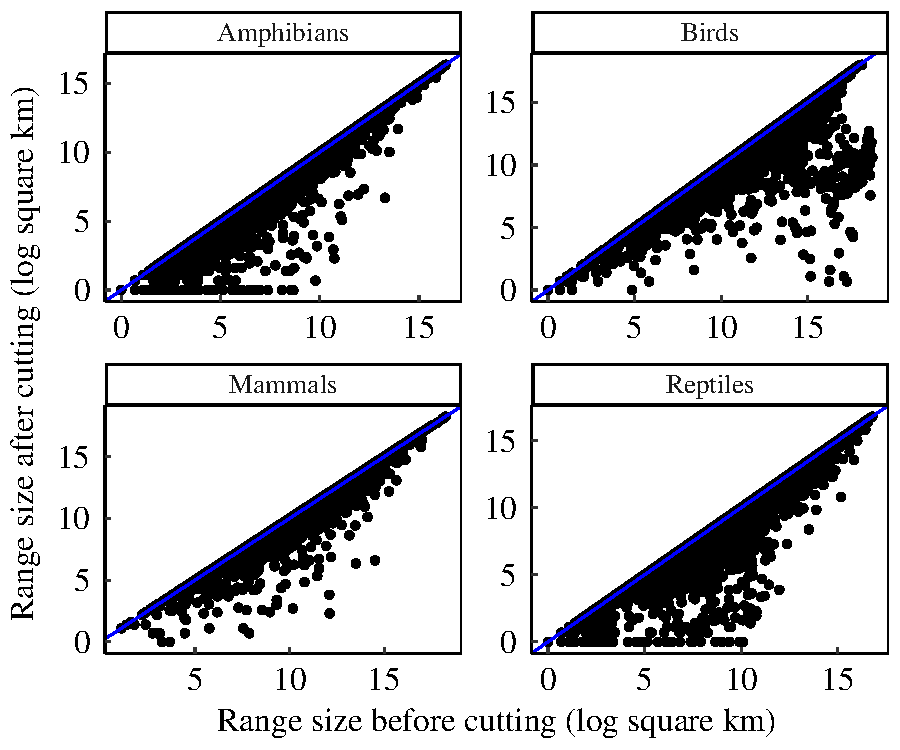
\includegraphics[scale=0.7]{Supporting/Chapter2/Figures/Rangesizes/RangeSizes_before_aftercuts}
\caption[]{\textbf{Range sizes before VS after cutting by altitudinal limits.}}
\label{}
\end{figure}

\pagebreak

\section{Impact of taxonomic corrections on trait coverage}

\begin{figure}[h!]
\centering
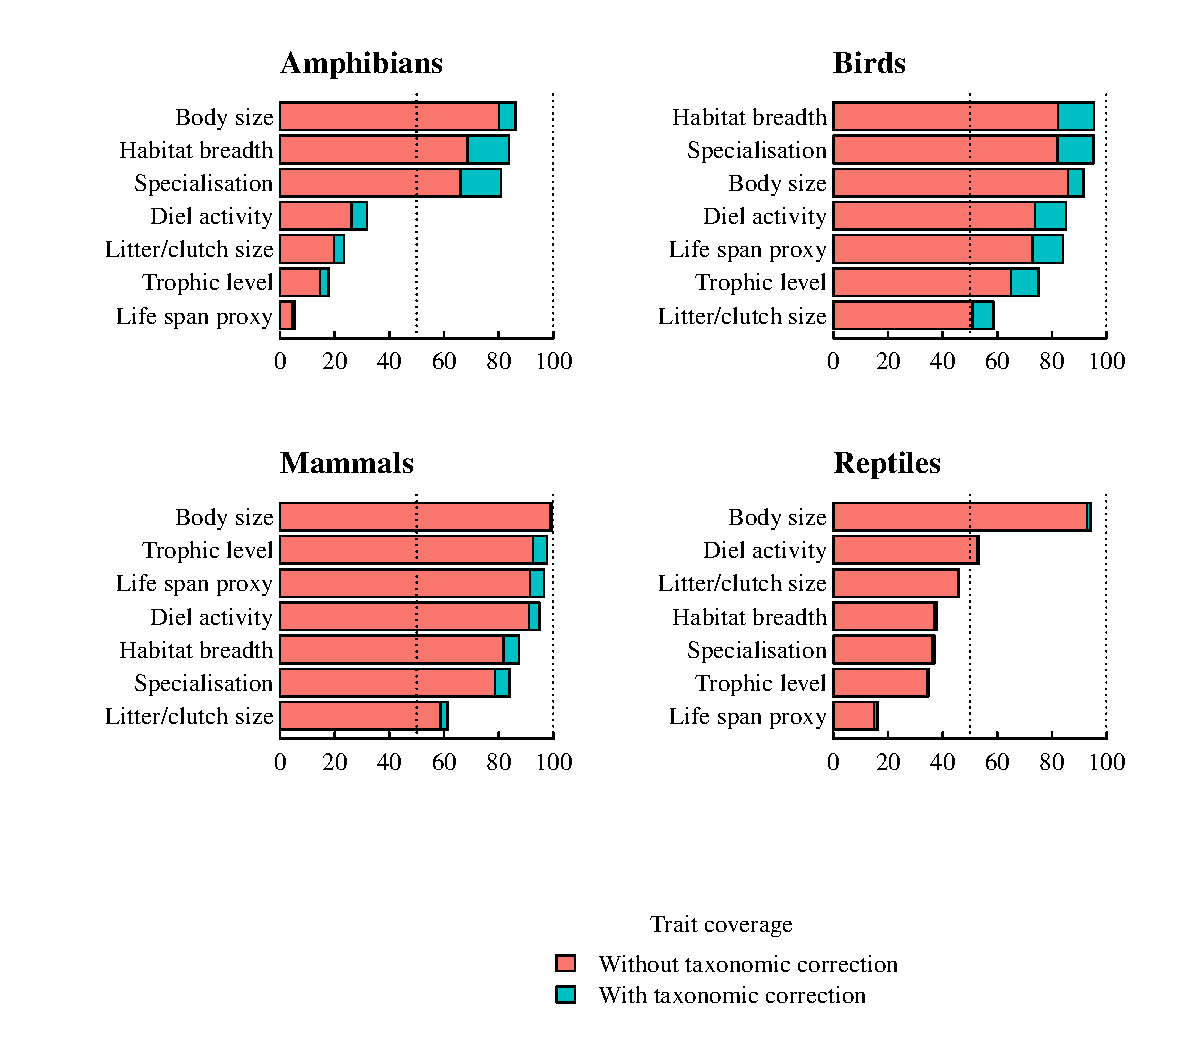
\includegraphics[scale=0.7]{Supporting/Chapter2/Figures/Coverage/DeltaCoverage}
\caption[]{\textbf{Trait coverage when no taxonomic correction is applied before matching sources by binomial names, versus when we apply the described procedure.} Identification of synonyms allowed to increase trait coverage in most cases.}
\label{}
\end{figure}

\newpage
\pagebreak

\section{Assemblage-level median, mean and standard deviation of trait completeness (maps)}

%% Median for all classes
\begin{figure}[h!]
\vspace*{-2cm}
\centering
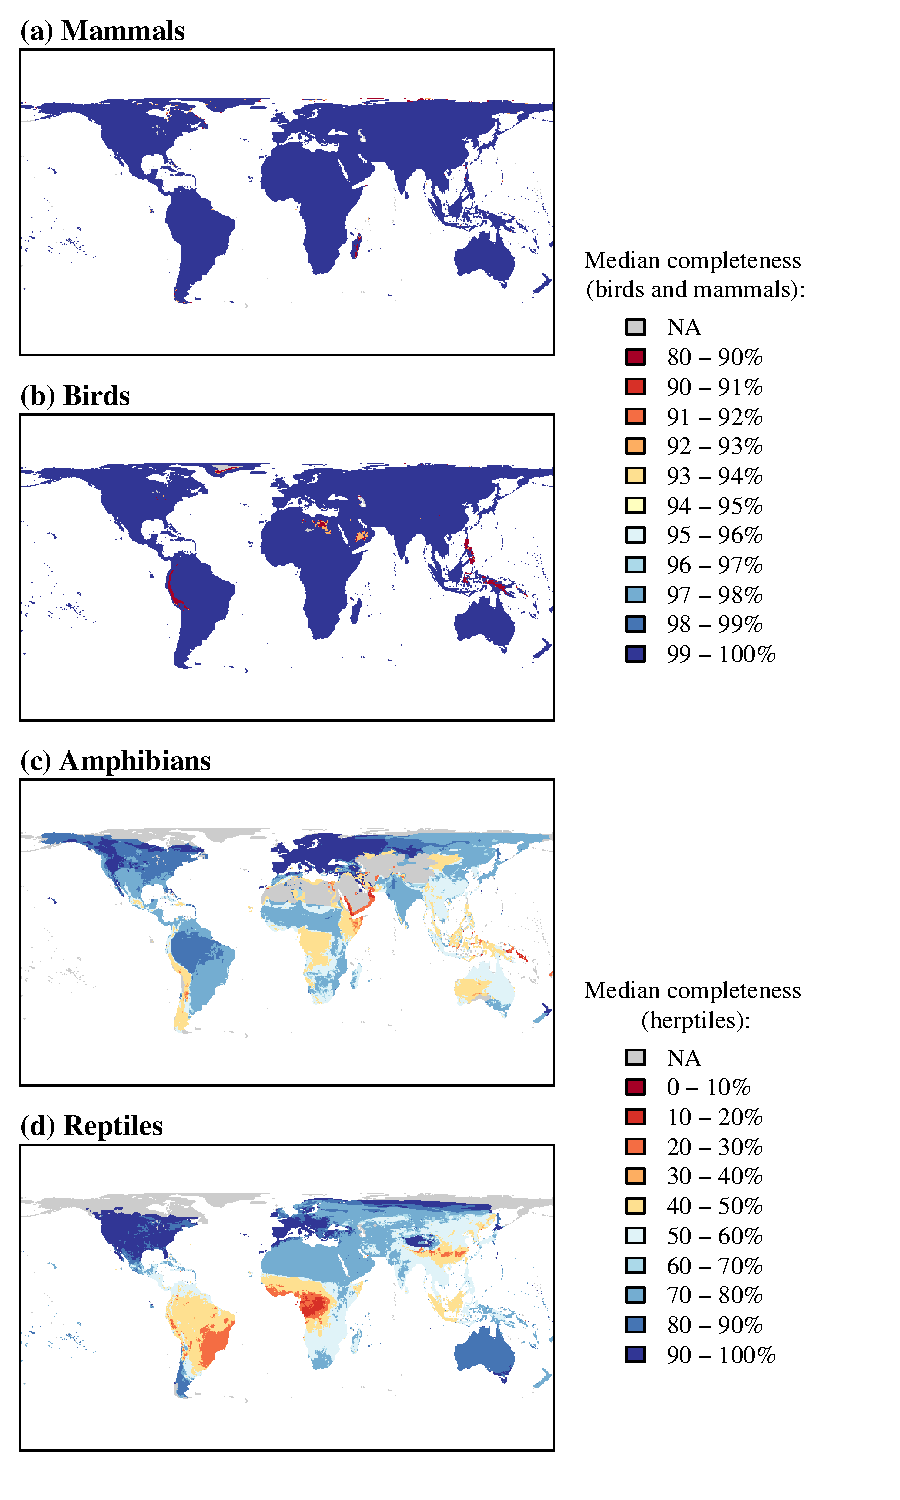
\includegraphics[scale=0.95]{Supporting/Chapter2/Figures/Maps/Median_map}
\caption[Spatial distribution of assemblage-level median trait completeness in herptiles.]{\textbf{Spatial distribution of  assemblage-level median trait completeness.} Note that the color breaks differ for mammals and birds and for herptiles.}
\label{}
\end{figure}

\newpage
%% Mean for all classes
\begin{figure}[h!]
\vspace*{-2cm}
\centering
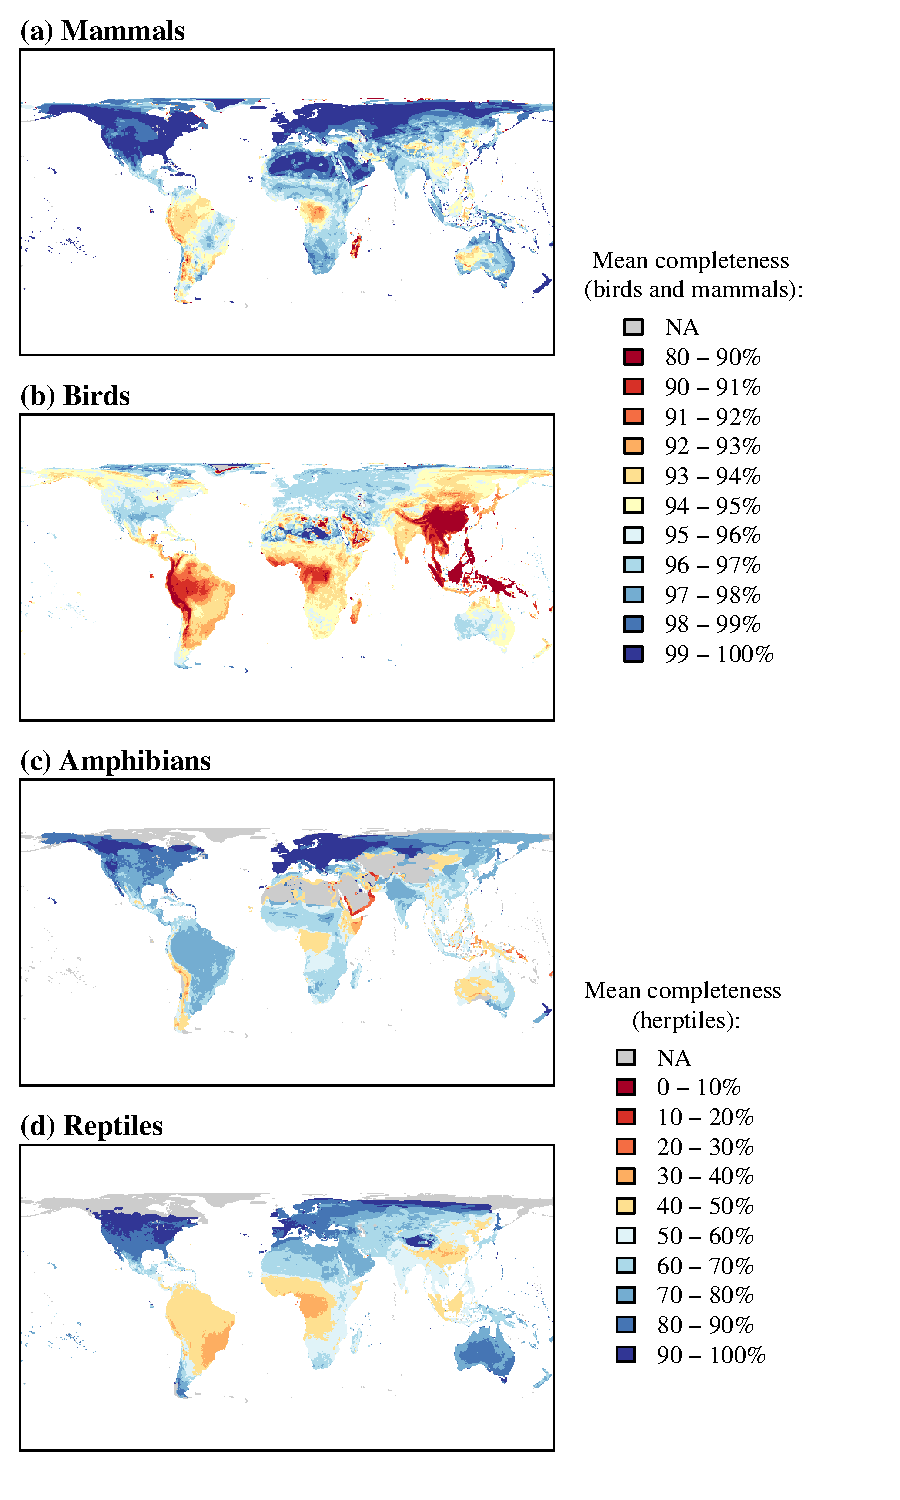
\includegraphics[scale=0.95]{Supporting/Chapter2/Figures/Maps/Mean_map_50k}
\caption[Spatial distribution of assemblage-level mean trait completeness in herptiles.]{\textbf{Spatial distribution of  assemblage-level mean trait completeness.} Note that the color breaks differ for mammals and birds and for herptiles.}
\label{}
\end{figure}

\newpage
%% Standard deviation for all classes
\begin{figure}[h!]
\vspace*{-2cm}
\centering
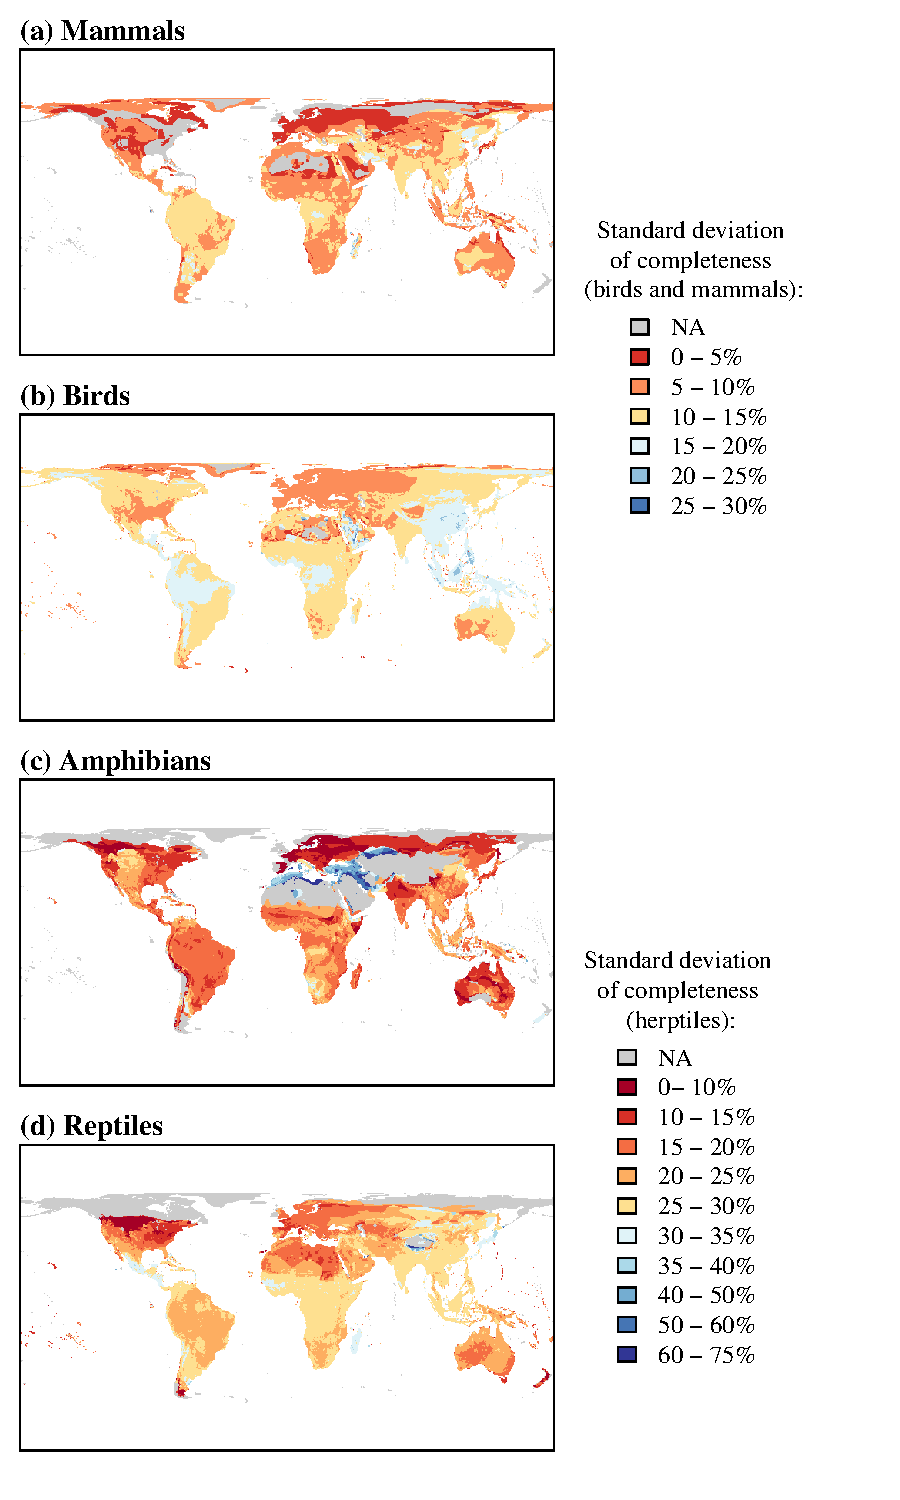
\includegraphics[scale=0.95]{Supporting/Chapter2/Figures/Maps/sd_map}
\caption[Spatial distribution of assemblage-level mean trait completeness in herptiles.]{\textbf{Spatial distribution of  assemblage-level standard deviation of trait completeness.} Note that the color breaks differ for mammals and birds and for herptiles.}
\label{}
\end{figure}


%% SD vs SR
\begin{figure}[h!]
\centering
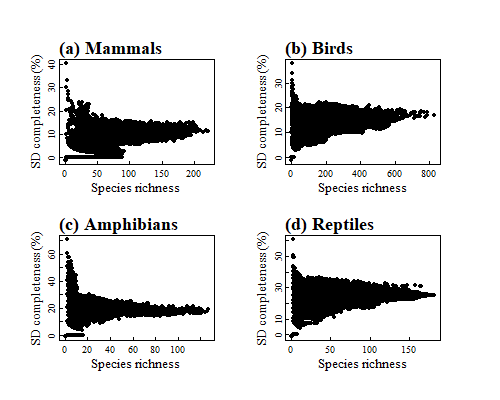
\includegraphics[scale=0.8]{Supporting/Chapter2/Figures/Maps/sd_SR.png}
\caption[]{\textbf{Assemblage-level species richness against standard deviation in completeness.}}
\label{}
\end{figure}

\clearpage
\newpage
\pagebreak

%%%%%%%%%%%%%%%%%%%%%%%%%%%%%%%%%%%%%%%%%%%
\clearpage
\newpage
\pagebreak

\begin{landscape}

\section{Phylogenetic patterns in trait completeness}


\begin{figure}[h!]
\centering
% [scale=1, clip, trim=110 200 100 200] #left bottom right top
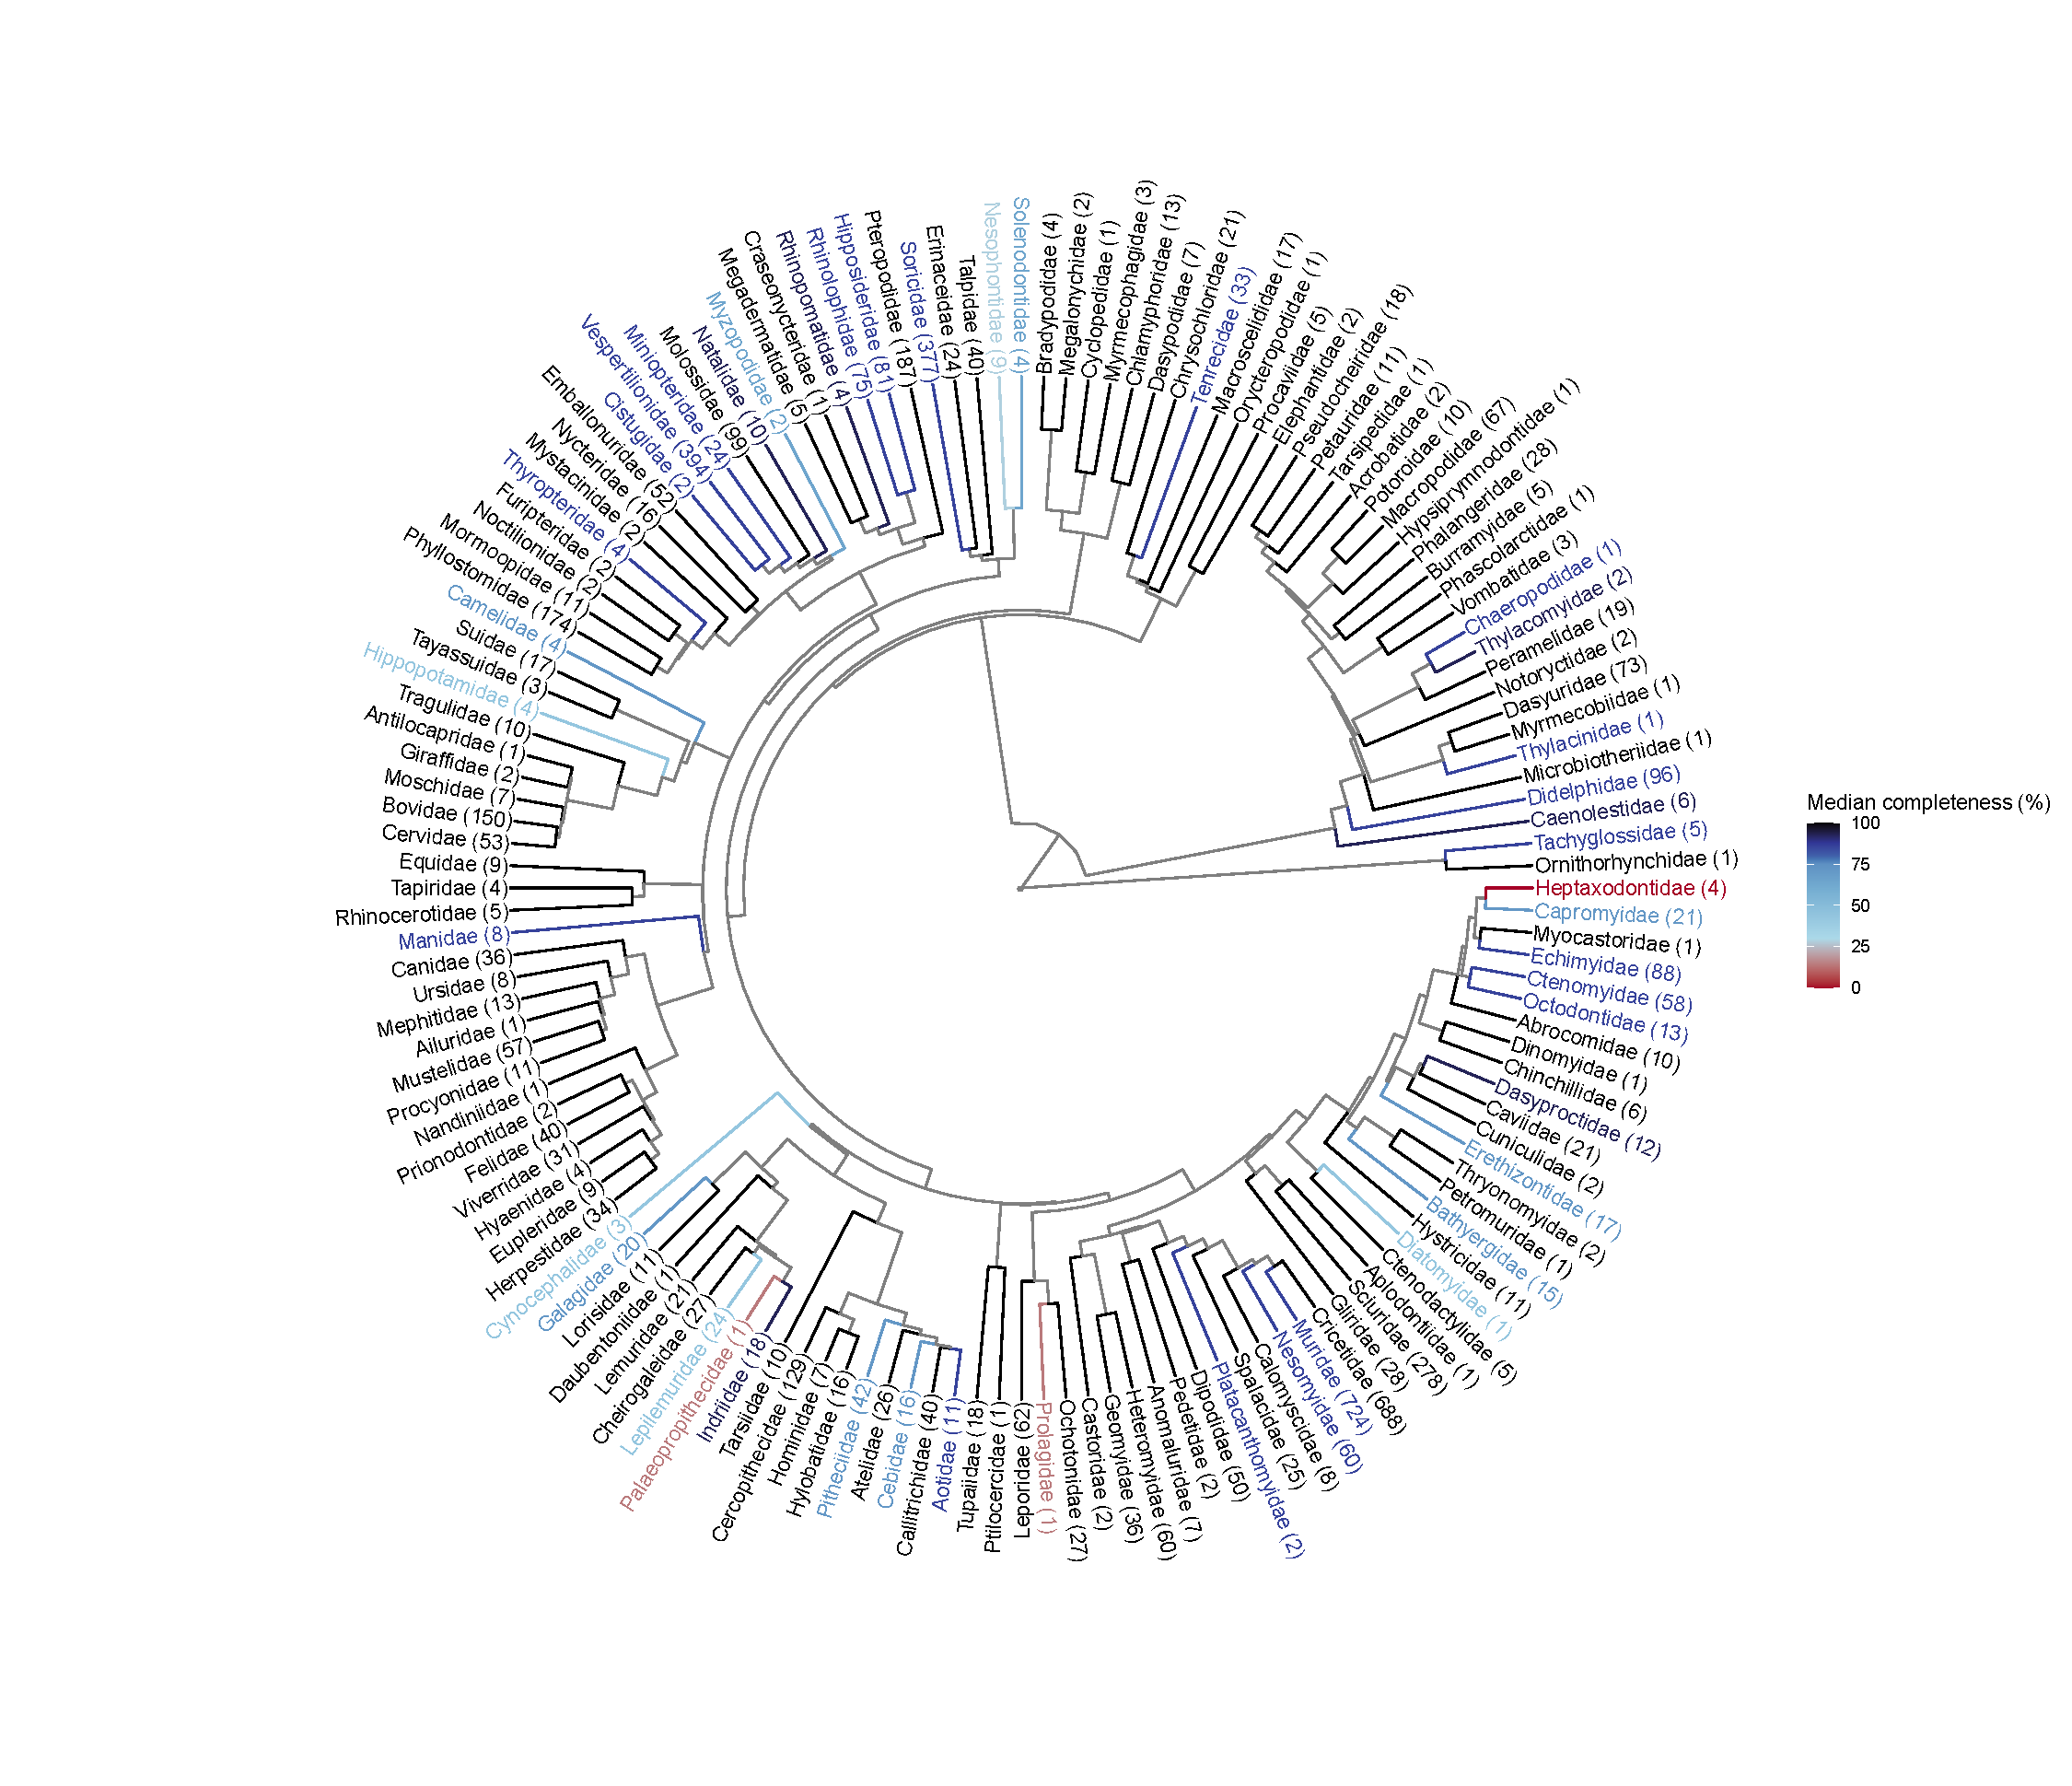
\includegraphics[scale=0.63, clip, trim=100 60 0 60]{Supporting/Chapter2/Figures/Phylogenies/Circular_mammals_V2}
\caption[Within-family median trait completeness in mammals]{\textbf{Within-family median trait completeness in mammals.}}
\label{}
\end{figure}

\newpage
\pagebreak
\vspace{-3cm}

\begin{figure}[h!]
\centering
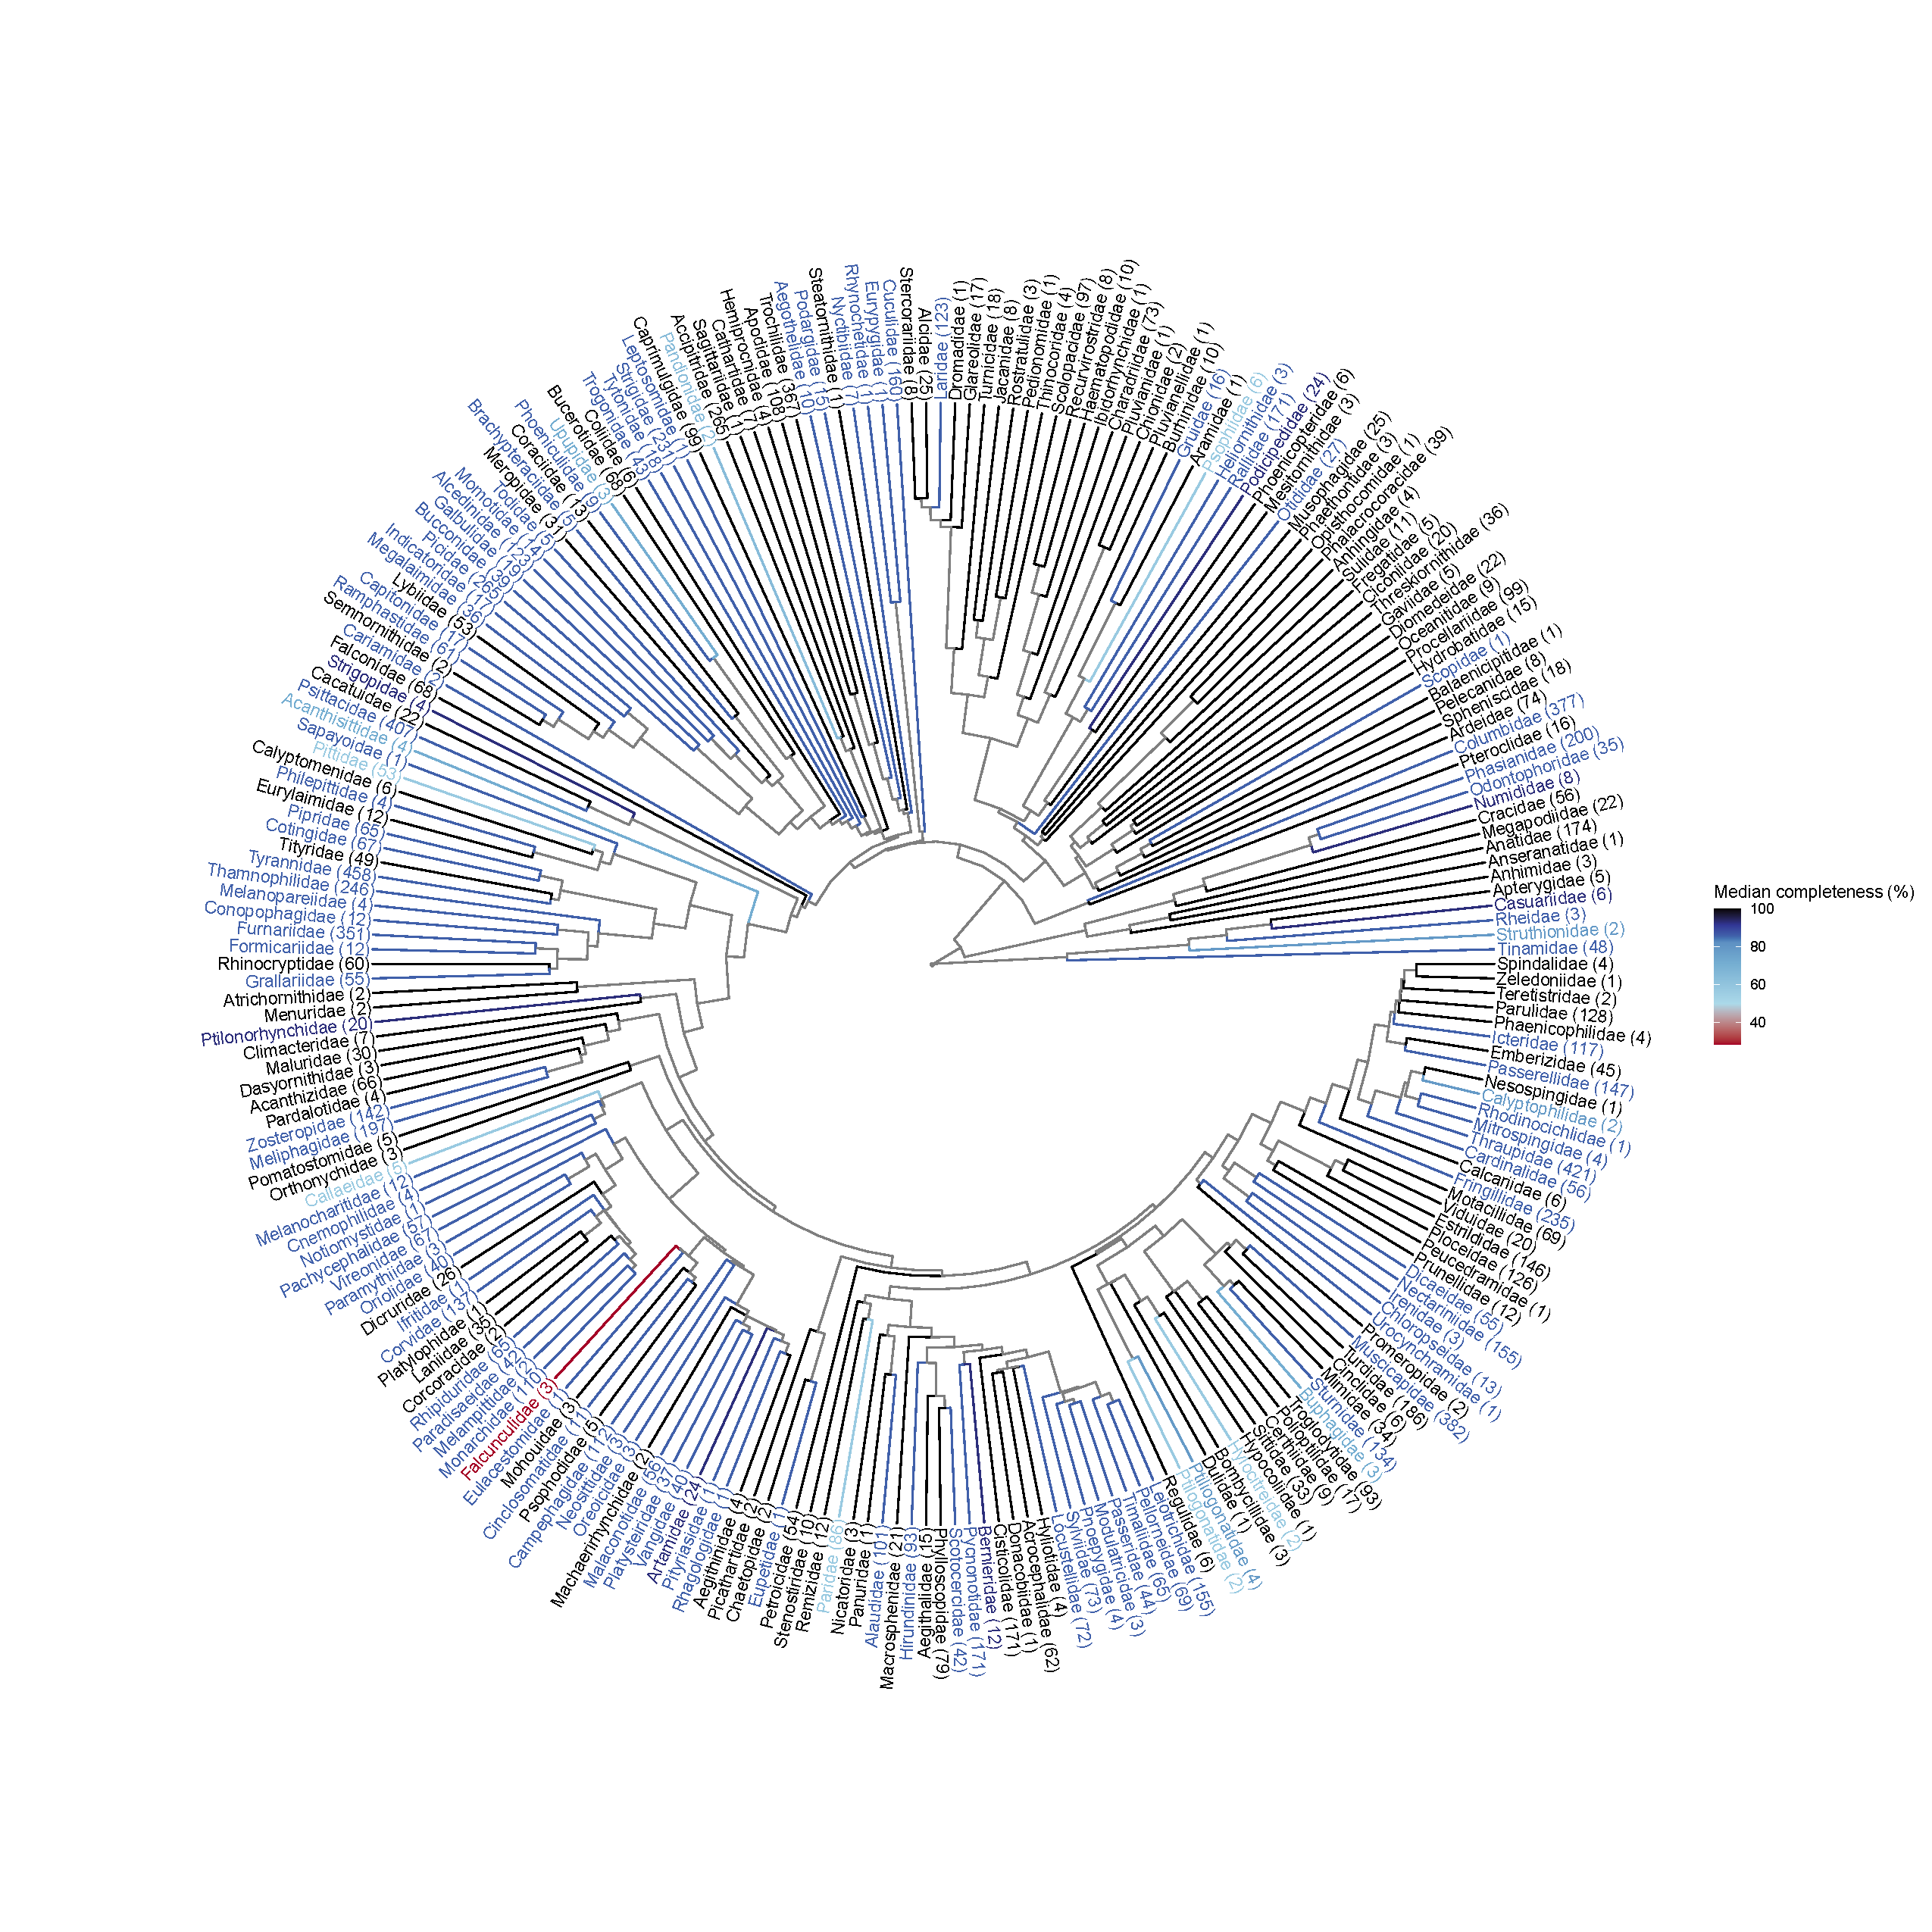
\includegraphics[scale=0.5,clip, trim=100 100 0 160]{Supporting/Chapter2/Figures/Phylogenies/Circular_birds_V2}
\caption[Within-family median trait completeness in birds]{\textbf{Within-family median trait completeness in birds.}}
\label{}
\end{figure}

\end{landscape}


\newpage
\pagebreak

\begin{figure}[]
\centering
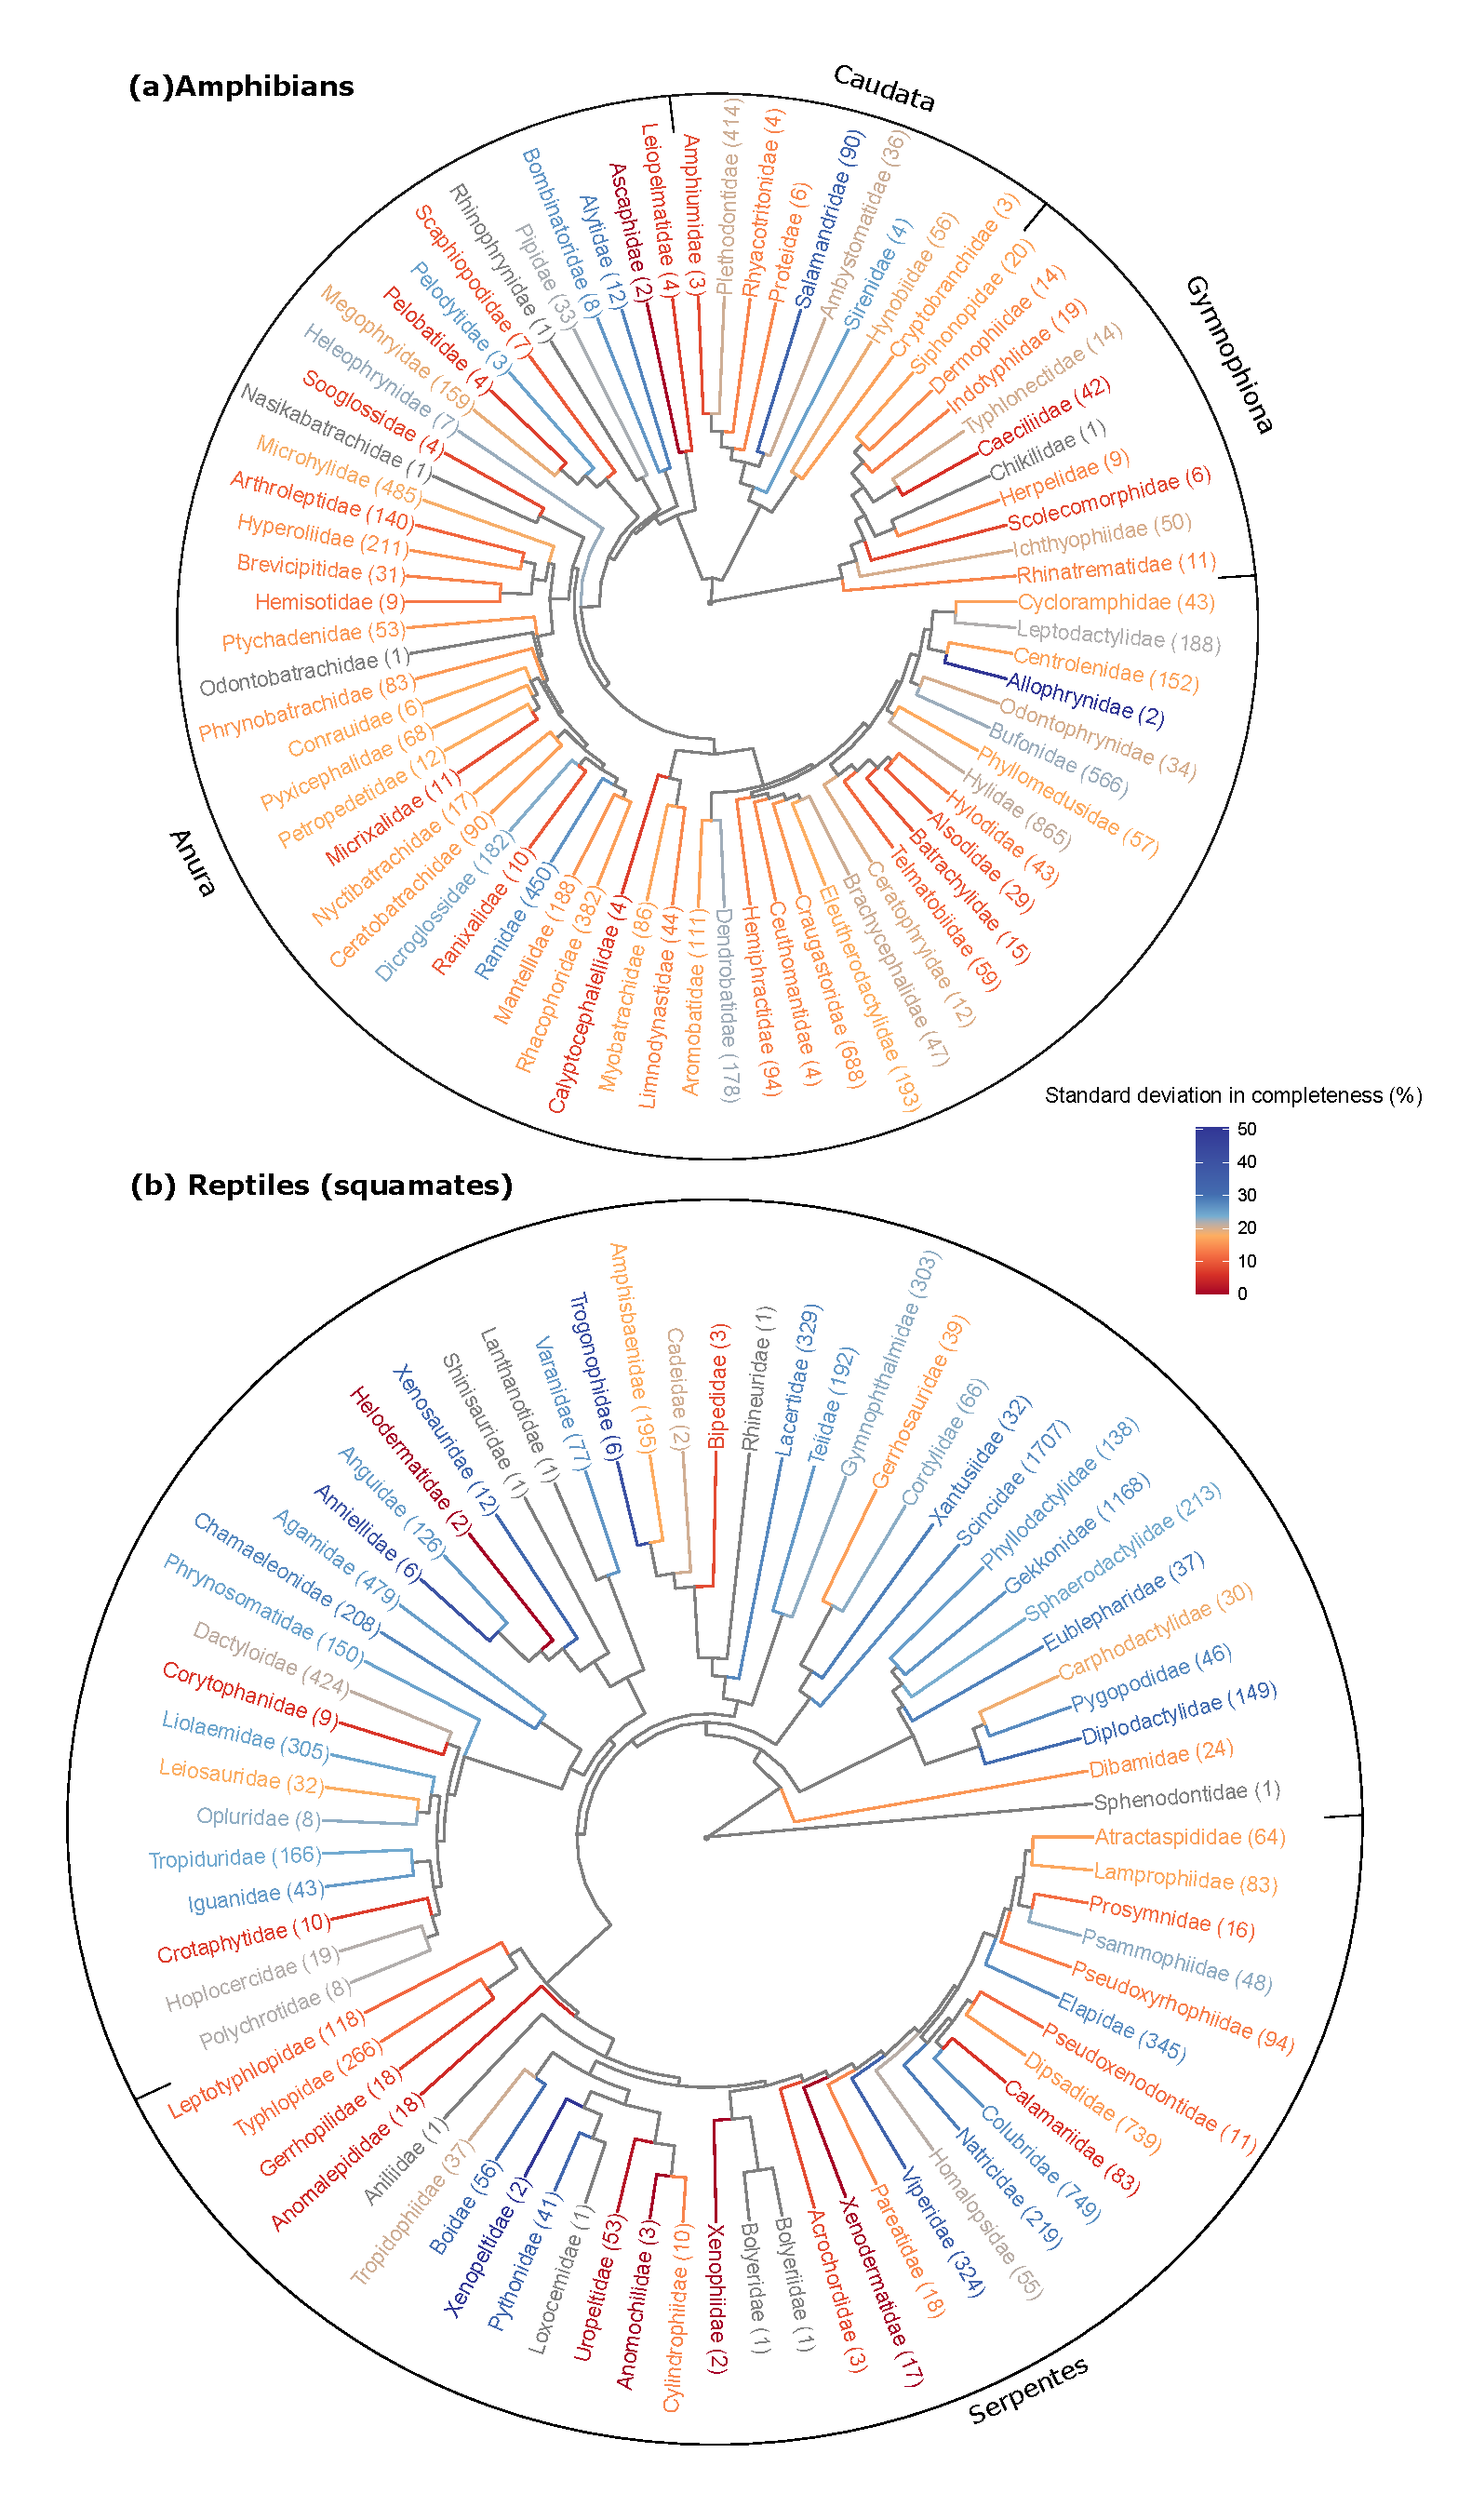
\includegraphics[scale=0.5, clip, trim=0 0 0 0]{Supporting/Chapter2/Figures/Phylogenies/Circular_herptiles_SD}
\caption[Within-family standard deviation in completeness.]{\textbf{Within-family standard deviation in completeness (herptiles).}}
\label{}
\end{figure}

\newpage
\pagebreak

\begin{figure}[h]
\centering
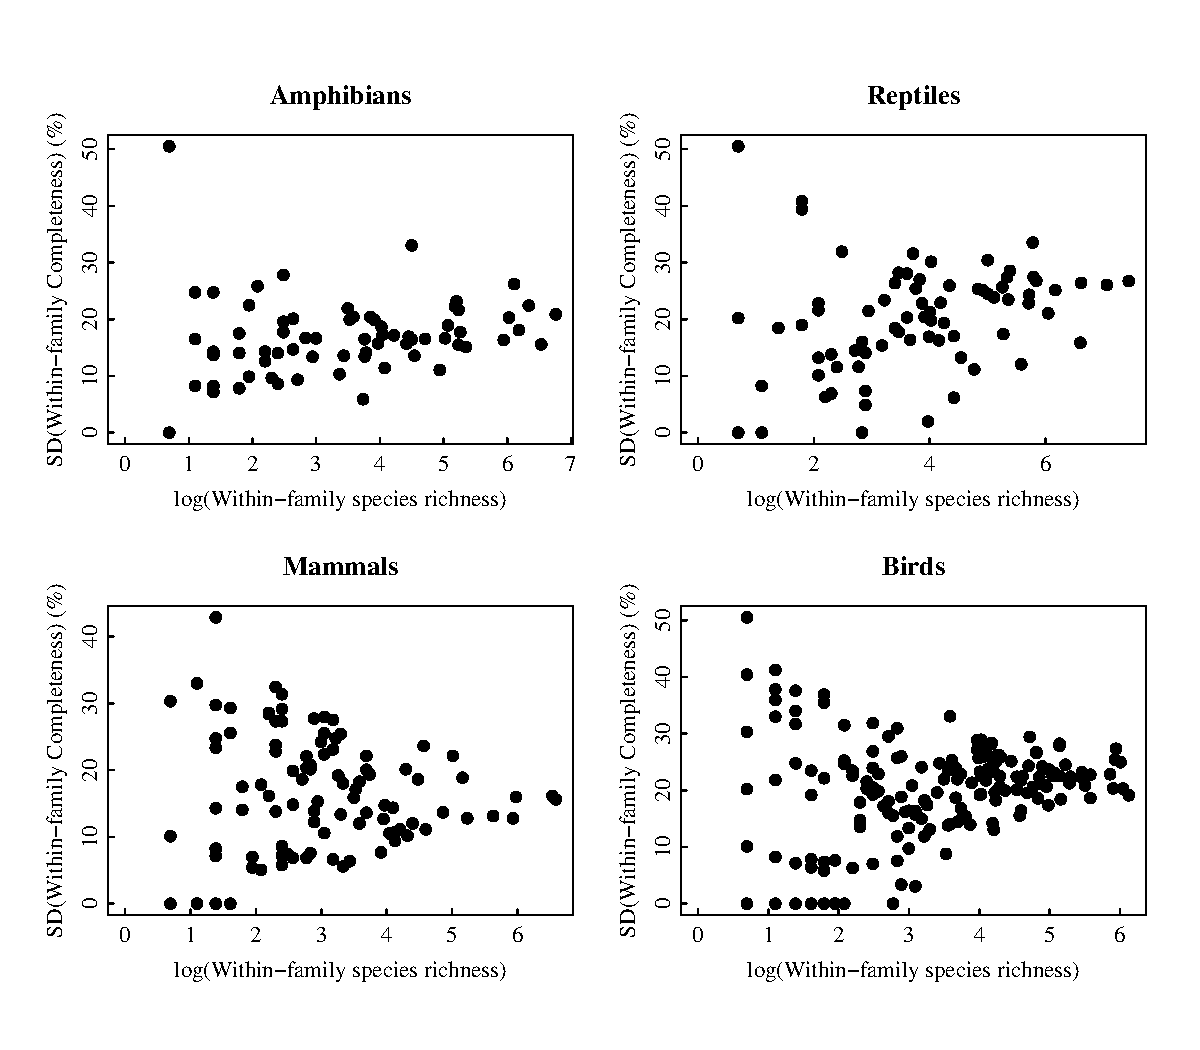
\includegraphics[scale=.6]{Supporting/Chapter2/Figures/Phylogenies/SD_VS_SR}
\caption[]{\textbf{Within-family species richness against the within-family standard deviation of completeness.}}
\label{}
\end{figure}

\clearpage
\section{Model coefficients for Range size against Number of sampled traits (Poisson model).}

%% New model coefficients:
\begin{table}[!htbp] \centering 
  \caption{\textbf{Coefficients of the model investigating whether species range size explained the number of sampled traits.} Class was added as an interacting predictor. The reference level for class is Mammals. The model was fitted using Poisson error distribution.} 
  \label{} 
\begin{tabular}{@{\extracolsep{5pt}} ccccc} 
\\[-1.8ex]\hline 
\hline \\[-1.8ex] 
 & Estimate & Std. Error & z value & Pr(\textgreater \textbar z\textbar ) \\ 
\hline \\[-1.8ex] 
Intercept & $1.678$ & $0.022$ & $76.809$ & $< 2e-16$ \\ 
log Range Size & $0.015$ & $0.002$ & $8.086$ & $6.16e-16$ \\ 
Class Birds & $$-$0.092$ & $0.028$ & $$-$3.350$ & $ 0.000809$ \\ 
Class Amphibians & $$-$0.689$ & $0.029$ & $$-$24.099$ & $< 2e-16$ \\ 
Class Reptiles & $$-$0.872$ & $0.027$ & $$-$31.856$ & $< 2e-16$ \\ 
log Range Size:Class Birds & $0.003$ & $0.002$ & $1.415$ & $0.157$ \\ 
log Range Size:Class Amphibians & $0.017$ & $0.003$ & $6.427$ & $ 1.30e-10$ \\ 
log Range Size:Class Reptiles & $0.026$ & $0.002$ & $11.159$ & $< 2e-16$ \\ 
\hline \\[-1.8ex] 
\end{tabular} 
\end{table}


\clearpage

\begin{table}[!htbp] \centering 
  \caption{\textbf{Coefficients of the model investigating whether species range size explained the number of sampled traits, \textit{using range maps not cut by altitudinal limits.}} Class was added as an interacting predictor. The reference level for class is Mammals. The model was fitted using Poisson error distribution.} 
  \label{} 
\begin{tabular}{@{\extracolsep{5pt}} ccccc} 
\\[-1.8ex]\hline 
\hline \\[-1.8ex] 
 & Estimate & Std. Error & z value & Pr(\textgreater \textbar z\textbar ) \\ 
\hline \\[-1.8ex] 
Intercept & $1.665$ & $0.023$ & $72.070$ & $< 2e-16$ \\ 
log Range Size & $0.015$ & $0.002$ & $8.167$ & $3.16e-16$ \\ 
Class Birds & $$-$0.110$ & $0.029$ & $$-$3.763$ & $0.0002$ \\ 
Class Amphibians & $$-$0.700$ & $0.030$ & $$-$23.721$ & $< 2e-16$ \\ 
Class Reptiles & $$-$0.928$ & $0.029$ & $$-$32.403$ & $< 2e-16$ \\ 
log Range Size:Class Birds & $0.004$ & $0.002$ & $1.840$ & $0.066$ \\ 
log Range Size:Class Amphibians & $0.018$ & $0.003$ & $6.564$ & $5.24e-11$ \\ 
log Range Size:Class Reptiles & $0.031$ & $0.002$ & $12.630$ & $< 2e-16$ \\ 
\hline \\[-1.8ex] 
\end{tabular} 
\end{table} 

\begin{figure}[h!]
\centering
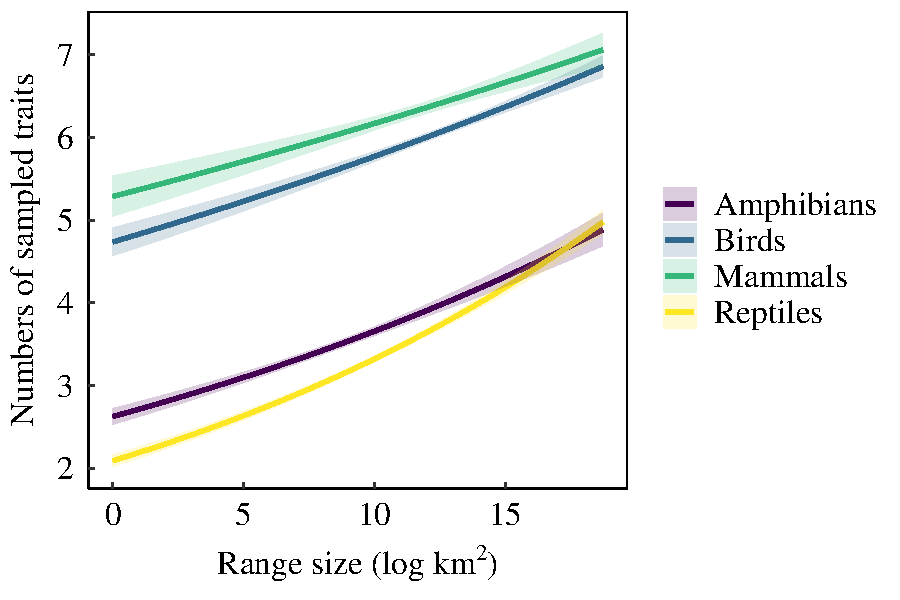
\includegraphics[scale=0.7]{Supporting/Chapter2/Figures/Plot_BeforeCuttingRS}
\caption[Relationship between number of sampled traits and geographical range size using distribution maps not cut by altitudina limits.]{\textbf{Relationship between number of sampled traits and geographical range size \textit{using distribution maps not cut by altitudinal limits}.} Models were fitted using a Poisson error distribution. Class was added as a predictor interacting with range size. Rates of increase were not significantly different for mammals and birds, but differed for reptiles and amphibians, with steeper rates of increase for reptiles overall. Cutting range maps by altitudinal limits had little effects on the results (Figure 4 in Main text).} 
\label{}
\end{figure}


\newpage
\pagebreak
\clearpage



% sample for spatial analyses
\section{Spatial models summaries}

% model summaries - amphibians
  \begin{table}[!htbp] \centering 
  \caption{Spatial model summary for amphibians. The spatial model was fitted to explain assemblage-level median completeness with species richness. Biogeographic realm was added as an interacting explanatory variable.} 
  \label{} 
\begin{tabular}{@{\extracolsep{5pt}} ccccc} 
\\[-1.8ex]\hline 
\hline \\[-1.8ex] 
 & Estimate & Std. Error & z value & Pr(\textgreater \textbar z\textbar ) \\ 
\hline \\[-1.8ex] Intercept - Realm: Afrotropic & $0.0738$ & $0.0064$ & $11.4908$ & $0$ \\ 
log(Species richness) & $$-$0.0025$ & $0.0017$ & $$-$1.4261$ & $0.1538$ \\ 
Realm: Australasia & $$-$0.0109$ & $0.0095$ & $$-$1.1453$ & $0.2521$ \\ 
Realm: Indo-Malay & $0.0455$ & $0.0119$ & $3.8294$ & $0.0001$ \\ 
Realm: Nearctic & $0.0441$ & $0.0082$ & $5.3905$ & $0.000000$ \\ 
Realm: Neotropic & $$-$0.0377$ & $0.0083$ & $$-$4.5538$ & $0.00001$ \\ 
Realm: Palearctic & $0.0047$ & $0.0067$ & $0.6992$ & $0.4844$ \\ 
log(Species richness):Australasia & $0.0018$ & $0.0038$ & $0.4789$ & $0.6320$ \\ 
log(Species richness):Indo-Malay & $$-$0.0147$ & $0.0039$ & $$-$3.7294$ & $0.0002$ \\ 
log(Species richness):Nearctic & $$-$0.0097$ & $0.0030$ & $$-$3.2003$ & $0.0014$ \\ 
log(Species richness):Neotropic & $0.0144$ & $0.0026$ & $5.6454$ & $0.000000$ \\ 
log(Species richness):Palearctic & $0.0109$ & $0.0029$ & $3.7358$ & $0.0002$ \\ 
\hline \\[-1.8ex] 
\end{tabular}  
\end{table} 

% model summary - reptiles
\begin{table}[!htbp] \centering 
  \caption{Spatial model summary for reptiles. The spatial model was fitted to explain assemblage-level median completeness with species richness. Biogeographic realm was added as an interacting explanatory variable.} 
  \label{} 
\begin{tabular}{@{\extracolsep{5pt}} ccccc} 
\\[-1.8ex]\hline 
\hline \\[-1.8ex] 
 & Estimate & Std. Error & z value & Pr(\textgreater \textbar z\textbar ) \\ 
\hline \\[-1.8ex] 
Intercept - Realm: Afrotropic & $0.2001$ & $0.0144$ & $13.9349$ & $0$ \\ 
log(Species richness) & $$-$0.0316$ & $0.0031$ & $$-$10.0547$ & $0$ \\ 
Realm: Australasia & $$-$0.1284$ & $0.0189$ & $$-$6.7851$ & $0$ \\ 
Realm: Indo-Malay & $$-$0.0453$ & $0.0263$ & $$-$1.7215$ & $0.0852$ \\ 
Realm: Neartic & $$-$0.0788$ & $0.0140$ & $$-$5.6366$ & $0.000000$ \\ 
Realm: Neotropic & $$-$0.0932$ & $0.0145$ & $$-$6.4425$ & $0$ \\ 
Realm: Palearctic & $$-$0.1030$ & $0.0131$ & $$-$7.8787$ & $0$ \\ 
log(Species richness):Australasia & $0.0386$ & $0.0046$ & $8.4019$ & $0$ \\ 
log(Species richness):Indo-Malay & $0.0124$ & $0.0061$ & $2.0397$ & $0.0414$ \\ 
log(Species richness):Neartic & $0.0346$ & $0.0038$ & $9.1601$ & $0$ \\ 
log(Species richness):Neotropic & $0.0220$ & $0.0034$ & $6.4231$ & $0$ \\ 
log(Species richness):Palearctic & $0.0286$ & $0.0033$ & $8.6153$ & $0$ \\ 
\hline \\[-1.8ex] 
\end{tabular}  
\end{table} 

\newpage
\pagebreak

\section{Trait coverage and taxonomic matching}

Here, we briefly explore the robustness of our work to taxonomic uncertainty by comparing trait coverage obtained with our procedure for taxonomic matching against trait coverage obtained when extracting synonyms from class-specific sources, which could contain more information, notably for herptiles. We aligned taxonomy again using the rangeBuilder R package, which allows the extraction of accepted names from class-specific sources. Overall, our results are robust to the use of different taxonomic backbones; the main conclusions are likely to be unaffected by taxonomic uncertainty.

\begin{figure}[h!]
\centering
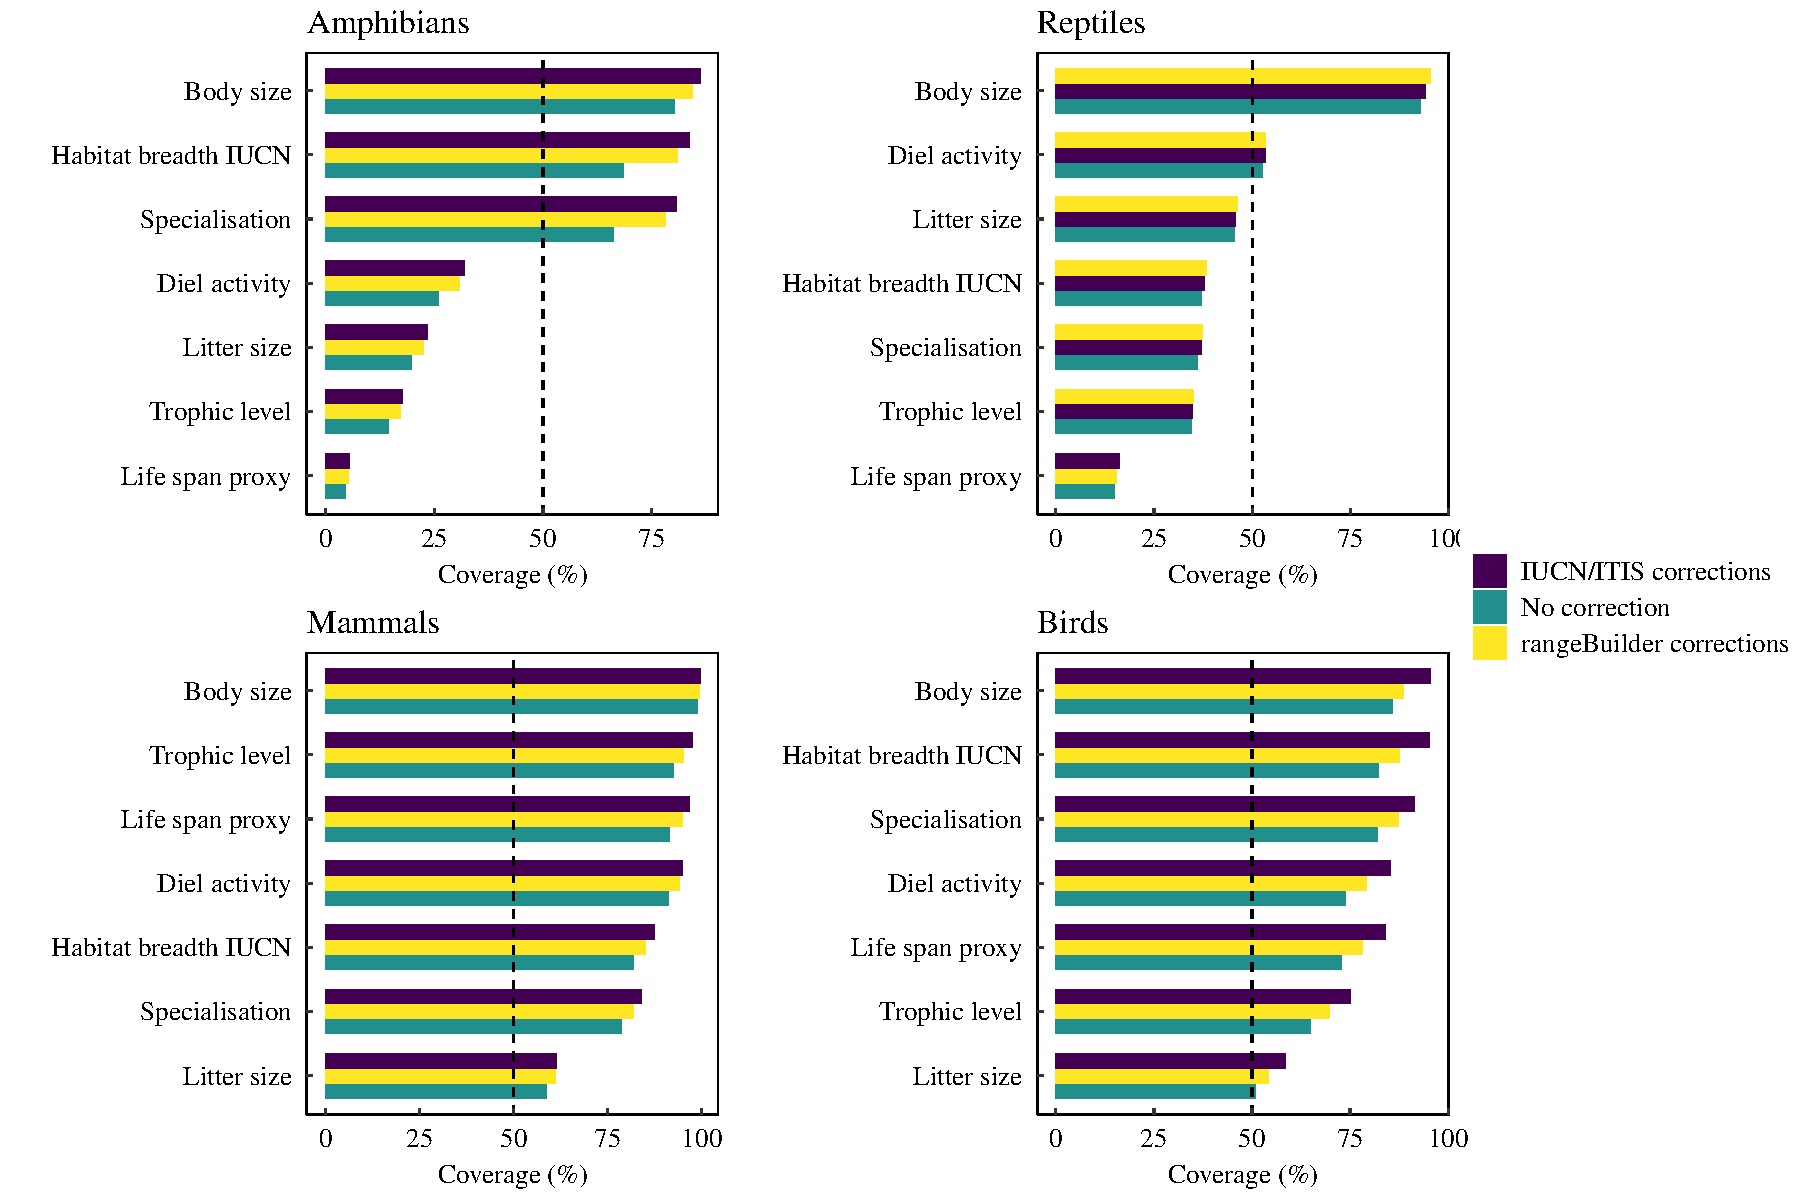
\includegraphics[scale=0.6]{Supporting/Chapter2/Figures/Coverage/DeltaCov_F3}
\caption[]{\textbf{Comparison of trait coverage among datasets corrected for taxonomy using the described procedure (purple bars), datasets corrected using the rangeBuilder package (extraction of synonyms from class-specific sources, yellow bars) and datasets where no taxonomic correction was applied when matching sources (green bars).}}
\label{}
\end{figure}